%!TEX root = ../dokumentation.tex
\chapter{Theory}

\section{Docker} 

To run applications on a cluster it is necessary to isolate these applications inside of a virtual container. Inside of these containers everything is available, what the application needs to get executed, but noting more. It is comparable to a \acs{VM} (\acl{VM}), but much more light weighted. This enables a very light deployment without unnecessary services or applications running in the background, which leads to a very performant execution. \textsuperscript{cmp.\cite{11}}

%https://ieeexplore.ieee.org/abstract/document/7093032/

Docker is such a technology for virtualization of containers. It provides a industry-leading container engine technology with an easy way to build containers with a Dockerfile and manage and run those containers easily on your local device. \textsuperscript{cmp.\cite{12}}

%https://www.docker.com/why-docker

The main difference between a container and a VM is the weight. While an average VM is hosting an operating system on top of a hypervisor on top of physical hardware. And on top of the OS of the VM the application is running. This affects the performance and the speed of the application in a very negative way, because a lot of unnecessary background proccesses are running. 

Docker solves this problem with a far more lightweight compute resource. The hypervisor of a docker container sits directly on the hosting operating system. This allows setting up several docker containers on only one phsyical machine and enables a high scalability. The differences between a VM and a docker container can be seen on the figure 2.1.1 below.

\begin{figure}[h]
\centering
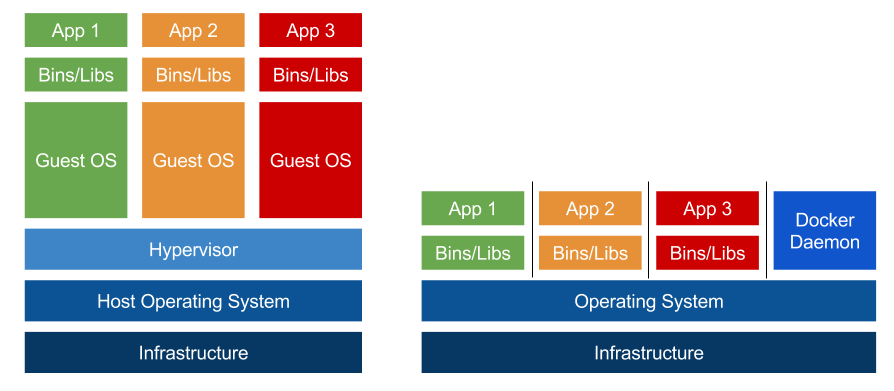
\includegraphics[width=\textwidth/5*4]{images/docker_vm_differences.png}

\textsuperscript{Figure 2.1.1 Comparison Docker container and VM}\\
\textsuperscript{Retrieved from \cite{13}}
\end{figure}
%https://blog.mikesir87.io/2017/05/docker-is-not-a-hypervisor/

On the left side the infrastructure of a VM can be seen, on the right side the infrastructure of a Docker container. Both needs a physical defice infrastructure and the host operating system. On a VM on this Host Operating System a Hypervisor is running and on this Hypervisor several Guest OS can be running. On those again the apps itself can be executed and the necessary libraries and binaries are running.

In case of a docker container those binaries and libraries are directly running on the operating system without the need of a hypervisor or a complete version of a Guest OS. This also enables the app to be running on top of that. The containers are isolated from each other in different namespaces and own network stacks. This means, that processes running within a container cannot see or interact with processes of other containers and they don't get privileged access to sockets or interfaces of other containers. \textsuperscript{cmp.\cite{14}}

%https://docs.docker.com/engine/security/security/

Additionally there is a Docker Daemon running in another process. The Docker Daemon has three main tasks - listening and processing API requests from the Docker client to run Docker commands, managing Docker objects (images, containers, volumes and networks) and parsing Dockerfiles for building docker images. \textsuperscript{cmp.\cite{15}}

%file:///C:/Users/IBM_ADMIN/Downloads/20170830_thesis_final.pdf

Those Dockerfiles contains the definition of a basic image, on which the new container should be based on, and then every operation to be executed to build the container. This includes copying necessary files, installing underlying services, compilers and libraries, setting up the environment, executing the commands to start the app and more. All those operations creating a new layer in the container. This leads a container to look like can be seen in the figure 2.1.2 with several layers with a unique id off different sizes based on one basic image like an Ubuntu image.

\begin{figure}[h]
\centering
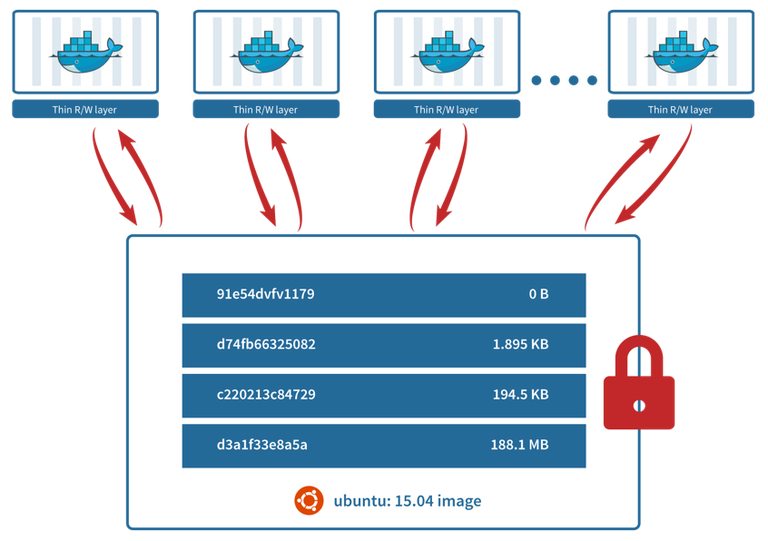
\includegraphics[width=\textwidth/5*3]{images/docker_layer.png}

\textsuperscript{Figure 2.1.2 Docker container layers}\\
\textsuperscript{Retrieved from \cite{16}}
\end{figure}
%https://adeeshfulay.wordpress.com/2017/09/08/understanding-docker-images-and-layers/

This has the advantage, that similar containers, which has equal parts as other, already existing layers, can mount the existing layers from the other container and don't need to build every container for their own again. This makes the build of the docker containers much faster and the single images are smaller, which is especially a great gain for continious inntegration. \textsuperscript{cmp.\cite{17}}

%https://tuhrig.de/layering-of-docker-images/

All in all Docker enables the creation of virtualized containers, in which applications can run isolated and independent from its environment. That's why it is a condition for deploying an application on a cluster, because there is no host operating system, on which the applications could be running otherwise.

%check?

\section{Kubernetes cluster solution}

One very common system for managing cluster systems as described in chapter 1.1 is \acl{K8s} - or short \acs{K8s}. Originally developed by Google and now maintained by the Cloud Native Computing Foundation, Kubernetes is an ``open-source platform for managing containerized workloads and services''.\textsuperscript{cmp.\cite{18}} For unterstanding what that means the concept of containers needs to be described first.

%https://kubernetes.io/docs/concepts/overview/what-is-kubernetes/

Containers are isolated, stand-alone packages of software, similar to processes. In those packages everything is included, which this piece of software needs, like runtime, libraries, settings and other system tools.  These containers have a completely different environment within themselves than outside. This environment includes for example network routes, dns settings and control group limits. This enables the possibility to share common resources and still be isolated from any other process as well as the host system. Thereby containers are always working the same, no matter on what system they run or in which environment.\textsuperscript{cmp.\cite{19}, \cite{20}}

%1 https://www.informatik-aktuell.de/entwicklung/methoden/kubernetes-architektur-und-einsatz-einfuehrung-mit-beispielen.html
%https://www.docker.com/what-container

Kubernetes is for an automating deployment, scaling and management of these containers within a cluster of nodes. Thereby a cluster consists of at least one master node and any number of worker nodes. Figure 2.1.1 shows the different services owned by master and worker nodes.

\begin{figure}[h]
\centering
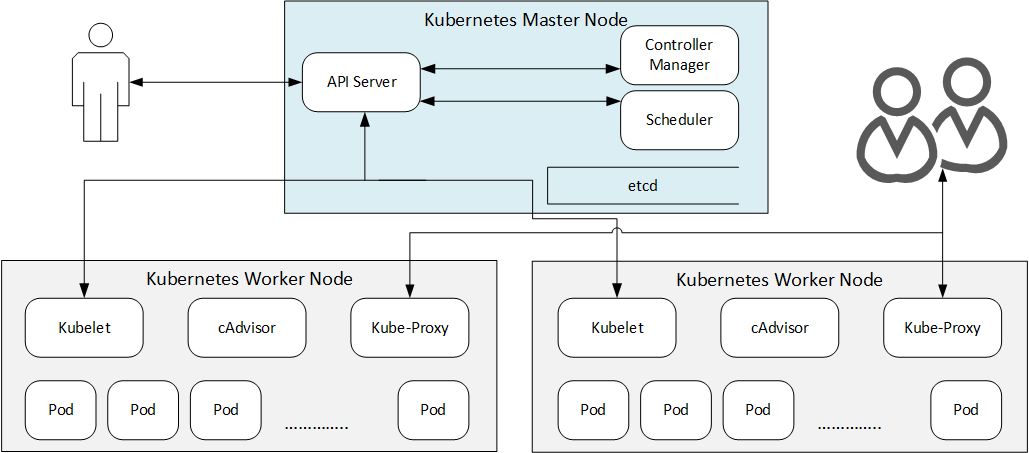
\includegraphics[width=\textwidth/5*3]{images/kubernetes_service_allocation.png}

\textsuperscript{Figure 2.1.1 Kubernetes allocation of services}\\
\textsuperscript{Based on retrieved information from \cite{19}}
\end{figure}

First there are several pods on each worker node. Pods are the smallest unit in Kubernetes. They contain one or more containers, which are deployed together on the same host. Thereby they can work together to perform a set of tasks.\textsuperscript{cmp.\cite{21}}%more?
%https://coreos.com/kubernetes/docs/latest/pods.html

On the master node there are an \acs{API} (\acl{API}) Server, a Controller Manager, a Scheduler and a key-value store called etcd.\textsuperscript{cmp.\cite{19}, \cite{22}}

The API Server is for clients to run their requests against. That means the API Server is responsible for the communication between Master and Worker nodes and for updating corresponding objects in the etcd. Also the authentication and authorization is task of the API Server. The protocol for the communication is written in \acs{REST} (\acl{REST}). For reacting on changes of clients there is also a watch mechanism implemented, which triggers an action after some specific changes, like the scheduler creating a new pod. This workflow is showed in figure 2.1.2.\textsuperscript{cmp.\cite{19}, \cite{22}}

\begin{figure}[h]
\centering
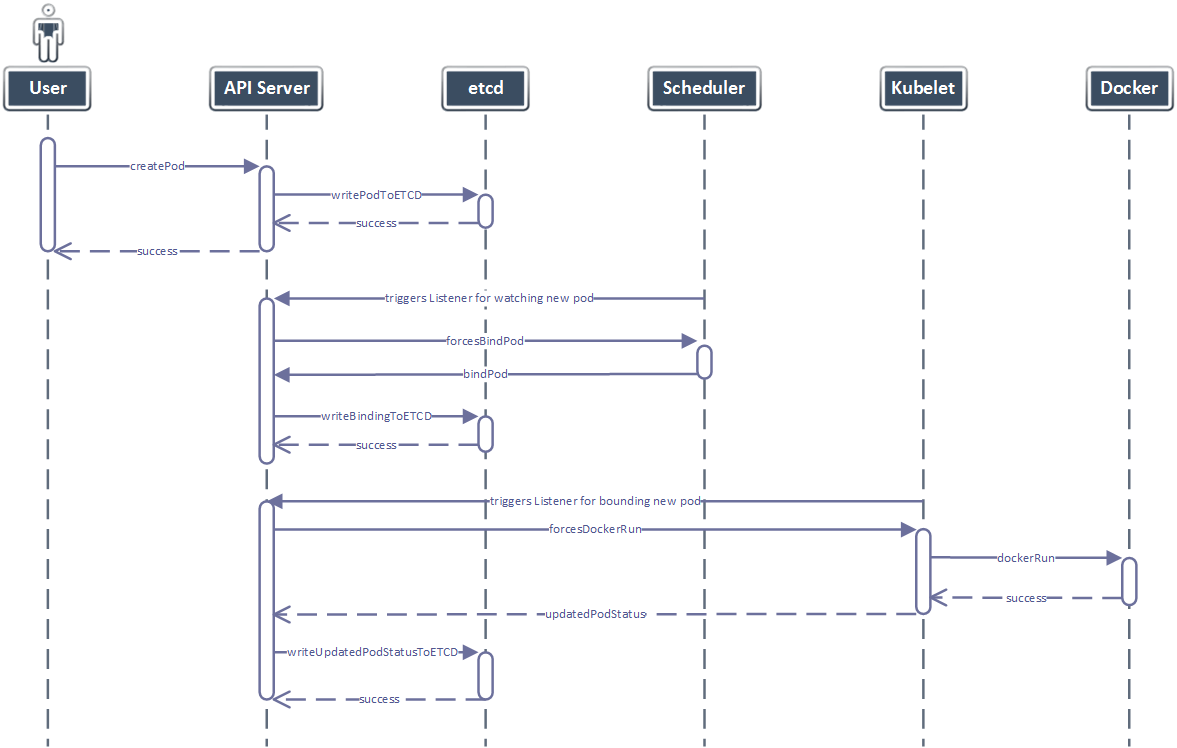
\includegraphics[width=\textwidth]{images/kubernetes_watcher_sequence.png}

\textsuperscript{Figure 2.1.2 Kubernetes API Server watcher sequence diagram}\\
\textsuperscript{Based on retrieved information from \cite{22}}
\end{figure}

There you can see the user creating a pod through a belonging request to the API Server. The API Server writes this change to the etcd. Afterwards the API Server recognizes a new pod in the etcd and invokes the Scheduler to create this new pod. What is the exact task of the scheduler is described later. After successfully creating and binding the new pod, the API Server writes this change to the etcd. Because of this change within the etcd the API Server invokes the kubelet, which is also described later in this chapter, of the corresponding node. This kubelet starts docker to create the containers of the pod. Kubelet responses with the new status of the pod, which is then written to the etcd by the API Server. After that the creation of the new pod is successfully finished.\textsuperscript{cmp.\cite{19}, \cite{22}}

The Controller Manager is a daemon, which embeds all of the Kubernetes controller. Examples for them are the Replication Controller or the Endpoint Controller. Those controllers are watching the state of the cluster through the API Server. Whenever a specific action happens, it performs the necessary actions to hold the current state or to move the cluster towards the desired state. For providing an example: If the Replication Controller recognizes, that one replication of a pod has been destroyed for some reason, it will take care of triggering the creation of a new replication.\textsuperscript{cmp.\cite{19}, \cite{22}}

The scheduler manages the binding of pods to nodes. Therefore it watches for new deployments as well as for old ones to create new pods if a new deployment is created or recreating a pod whenever a pod gets destroyed. The scheduler organizes the allocation of the pods within the cluster on the basis of available ressources of the pods. That means, that it always create pods, where the most resources are available, or reorganize the allocation if there is a change in the resource allocation of the cluster.\textsuperscript{cmp.\cite{19}, \cite{22}}%??

For example if we have four pods deployed on our cluster - as long as there are only two nodes, it allocates those four pods to the two nodes in pairs of two. As soon as there are more nodes connected, the scheduler recognizes free resources and reallocate the pods to these new nodes, so that we have one pod on each node.

The etcd is a key-value store, which stores the configuration data and the condition of the Kubernetes cluster. The etcd also contains a watch feature, which listens to changes to keys and triggers the API server to perform all necessary actions to move the current state of the cluster towards the desired state.\textsuperscript{cmp.\cite{19}, \cite{22}}

The worker node consists of a Kubelet, a cAdvisor, a Kube-Proxy and - as mentioned before - several Pods. 

The kubelet needs to be used if a new pod should be deployed. Then it gets the action to create all needed containers. For that it uses Docker to create them. Afterwards it combines some containers into one pod. Conainers in one pod are always started and stopped together. This pod will then be deployed on the node, on which the kubelet is located.\textsuperscript{cmp.\cite{19}, \cite{22}}

The cAdvisor measures the usage of CPU-resources as well as demanded memory on the node, on which it is located, and notifies the master about it. Based on those measurements the scheduler allocates the pods within the cluster to ensure the best possible allocation of resources.\textsuperscript{cmp.\cite{19}, \cite{22}}

The kube-proxy is a daemon, that runs as a simple network proxy to provide the possibility of communicating to that node within the cluster. Additionally it runs a load balancer for the services on that node.\textsuperscript{cmp.\cite{19}, \cite{22}}

Through this architecture Kubernetes enables different possibilities to deploy pods within the cluster. The simplest one is to deploy a specific pod directly. This deploys the pod described in a file, but it doesn't ensure the failure safety. That means if the pod gets destroyed for some reason, no matter if it has been destroyed by accident or intended, it won't be recreated and deployed again automatically. 

Another possibility is to create a deployment. Therefore the image has to be embedded within a replicaset and this replicaset within a deployment. If this deployment is created, it will automatically create every pod of the replicaset. If one pod gets terminated, no matter if manually or because of an error, it will be directly recreated and deployed. This also enables dynamical rolling updates for deploying a new version of a pod.\textsuperscript{cmp.\cite{19}, \cite{23}}

Additionally Services can be created on a cluster. Services are used to enable the usage of pods from outside the container. Therefore it gets the pod from the targetPort of the belonging node and creates a random port on this node. This port serves as endpoint for the LoadBalancer. Through this, every pod on the cluster can now communicate with this pod. For a communication to the outside of the cluster this port needs to be exposed afterwards, for example with an ingress. \textsuperscript{cmp.\cite{19}, \cite{23}}

This is how Kubernetes ensures High Availability as well as Load Balancing at the same time. Through the possibility of replicate every pod several times it is ensured that whenever one pod fails for some reason, another is already prepared to help out and take over the job. Even the master can and should be replicated to ensure a functional system, even if one master has been destroyed.\textsuperscript{cmp.\cite{19}, \cite{23}}

%1
%2
%https://deis.com/blog/2016/kubernetes-overview-pt-1/

All in all Kubernetes combines all the benefits of cluster applications in one software. High availability as well as load balancing is guaranteed and it also ensures a high scalability, rolling updates and auto-scaling. This makes Kubernetes one of the most flexible and fastest cluster systems. In exchange for that flexibility it is more difficult to set it up compared to other cluster systems, because you have to do it all on your own. But only that way it can be ensured, that it runs fast and flexible in the same time, which is the reason for Kubernetes being so popular.\textsuperscript{cmp.\cite{24}, \cite{25}}

%https://platform9.com/blog/kubernetes-docker-swarm-compared
%https://www.redhat.com/de/topics/containers/what-is-kubernetes ???

\section{Apache Kafka}

For a scalable system with a potential of a huge amount of requests every second a realtime streaming platform is necessary. This platform needs to be able to consume messages without blocking the producer even for a second and to produce messages without the need to know the final addressee. Such a streaming platform is Apache Kafka, originally developed by LinkedIn and managed by Apache Software foundation with Open Source license. \textsuperscript{cmp.\cite{26}}

%https://books.google.de/books?hl=de&lr=&id=qS9eAQAAQBAJ&oi=fnd&pg=PT6&dq=apache+kafka&ots=ZtW04yIrqG&sig=b2ix-I9ck0zGcM2LfA-zYhEbP9g#v=onepage&q=apache%20kafka&f=false

Apache Kafka thereby characterizes through the possibilities of a very high throughput, so that it can support millions of messages per second, and real time functionalities, which means, that every produces message is immediately visible to consumer threads. Additionally Kafka supports multiple client systems from different platforms like Java, Python, PHP and more and also it supports distribution over a cluster of consumer machines while maintaining its ordering semantics. \textsuperscript{cmp.\cite{26}}

%%https://books.google.de/books?hl=de&lr=&id=qS9eAQAAQBAJ&oi=fnd&pg=PT6&dq=apache+kafka&ots=ZtW04yIrqG&sig=b2ix-I9ck0zGcM2LfA-zYhEbP9g#v=onepage&q=apache%20kafka&f=false

For the realization of these characteristics the architecture of Kafka looks like can be seen in figure 2.3.1. Any amount of producers can produce messages to the Kafka brokers. For that it uses a key-value pair as well as a topic, to which it will produce the message. The broker then stores the message with a timestamp to the topic. \textsuperscript{cmp.\cite{26}}

%%https://books.google.de/books?hl=de&lr=&id=qS9eAQAAQBAJ&oi=fnd&pg=PT6&dq=apache+kafka&ots=ZtW04yIrqG&sig=b2ix-I9ck0zGcM2LfA-zYhEbP9g#v=onepage&q=apache%20kafka&f=false
\begin{figure}[h]
\centering
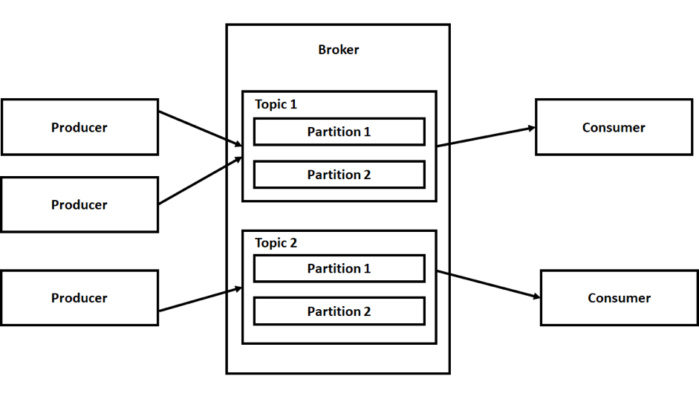
\includegraphics[width=\textwidth/5*4]{images/kafka_architecture.png}

\textsuperscript{Figure 2.3.1 Apache Kafka Architecture}\\
\textsuperscript{Retrieved from \cite{27}}
\end{figure}
%https://www.infoworld.com/article/3215165/application-development/how-to-use-apache-kafka-messaging-in-net.html

One broker contains several topics, which can be considered as a logical collection of messages. The topics can be divided into one or more partitions. Those partitions are distributed across multiple brokers, which enabled Kafkas abilitiy for dynamically scaling. For that all brokers are connected to one, big cluster of brokers. This cluster is then managed by a Zookeeper Client, which maintains the confguration information across its nodes. \textsuperscript{cmp.\cite{27}}

%https://www.infoworld.com/article/3215165/application-development/how-to-use-apache-kafka-messaging-in-net.html

Consumer read from Kafka topics. This means they are listening on a topic and as soon as a new message is produces to it, the consumer recognizes that and reads the newly produced message.

This makes Apache Kafka to a simple-to-use real time streaming platform, which is very scalable, performant and stable through its cluster structure, which enables replications, distribution and partitioning. \textsuperscript{cmp.\cite{28}}

% http://cloudurable.com/blog/kafka-architecture/index.html

\section{Open Source Routing Machine}

One requirement of a car sharing app is of course the routing of a vehicle to its given destination. In the drl car sharing app this is done with \acs{OSRM} (\acl{OSRM}), which is designed for use with OpenStreetMaps.

Before calculating the shortest path from A to B OSRM needs an Open Street Map in osm.pbf format. This map needs then to be prepared, which includes extracting the map, partitioning the graph recursively into cells and customize it by calculating routing weights for all cells. When extracting the map it can also include a vehicle profile, which initialized the map with knowledge about which paths can be taken by the specific vehicle and which cant. For example some routes are only accessible by bikes or pedestrians, others can only be accesses with a car.  \textsuperscript{cmp.\cite{29}, \cite{30}}

%https://github.com/Project-OSRM/osrm-backend
%https://med.mahidol.ac.th/ceb/sites/default/files/public/pdf/stata_journal/sj16-2.pdf#page=178

For the calculation of the route OSRM describes the map as a graph. In a simple model intersections are described as entities and the roads are used as connections between those entities. Those connections are called edges. Every edge gets a weight added, which denotes the cost to traverse the connection, for example time or distance. The goal is then to calculate the path with the minimum overall weight, when all connections leading from the origin edge to the destination edge are summed together. \textsuperscript{cmp.\cite{31}}

%https://blog.mapbox.com/smart-directions-powered-by-osrms-enhanced-graph-model-3ae226974b2

After the visualization of the road network as a weighted graph, the shortest path needs to be found. For that OSRM uses the Dijkstra's Algorithm. This algorithm looks for every node connected to the source node and stores the weight of the connecting edge. In case there are several connecting edges it takes the edge with the smallest weight. Then it continues recursively and looks for every node connected to the new nodes. Every node, for which the connections have been calculated, are added to a set ``visited''. The recursion stops when it reaches a node, which is already in the ``visited'' set. When visiting a new node it stores this to a path log and summing the weight of all the edges it took on its way. This way it calculates the distance between every node by summing the weight of every connection from the origin node to the destination node and storing all nodes visited on the path to it.  \textsuperscript{cmp.\cite{32}}

%file:///C:/Users/IBM_ADMIN/Downloads/algorithms%20(1).pdf

This is done for every node of the map when preparing the map for its use. So there is every possible path stored from any node to any other node. When looking for the shortest path OSRM only needs to look for every path leading from the origin node to the destination node and picks the smallest one. The car sharing app uses this routing machine for calculating the shortest path for the vehicles to its destinations.

\section{Mongo Database}

For a performant and scalable processing of huge amounts of data on a Cloud platform a special database technology is necessary. A very popular database technology for that purpose is \acs{MongoDB} (\acl{MongoDB}). MongoDB was developed by the compand 10gen since 2007 and the name Mongo stands for ``Humongous''.  \textsuperscript{cmp.\cite{33}}

%https://www.iks-gmbh.com/files/pdf/alvermann_JS_01_11.pdf

MongoDB characterizes through its simple data replication and scalability. For that MongoDB consists out of a cluster of server, which can be easily extended, so that there is no need for upgrading single servers for scaling the database. Additionally MongoDB is a lot faster than relational databases. As an example in figure 2.5.1 it can be seen a comparison between update requests of MongoDB and traditional \acs{SQL} (\acl{SQL}) requests at different scales.

\begin{figure}[h]
\centering
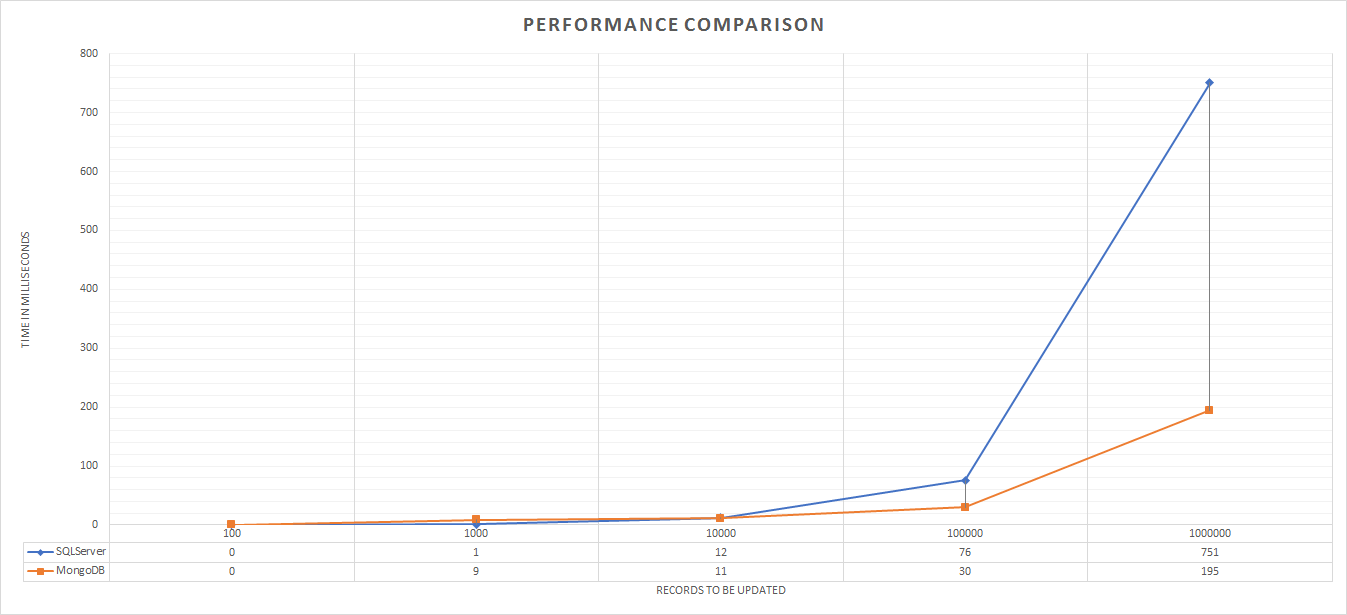
\includegraphics[width=\textwidth]{images/mongo_sql_comparison.png}

\textsuperscript{Figure 2.5.1 Performance comparison Mongo and SQL}\\
\textsuperscript{Based on retrieved information from \cite{34}}
\end{figure}

%%https://www.researchgate.net/figure/Comparing-the-performance-of-updating-the-records-at-different-scales-times-are-in_fig6_281629941

The x axis is the scale of records to be updated and the y axis shows the time it needs in milliseconds. With a small amount of requests the difference is quite low, but as larger the scale get, the greater the difference between those technologies get. With a scale of 100000 records MongoDB is already more than twice as fast as a SQL Server (30 milliseconds for MongoDB and 76 milliseconds for MySQL). When increasing the scale to 1000000 records MongoDB is almost four times faster than SQL.  \textsuperscript{cmp.\cite{34}}
%%https://www.researchgate.net/figure/Comparing-the-performance-of-updating-the-records-at-different-scales-times-are-in_fig6_281629941

Different to SQL databases Mongo stores its data as documents instead of relational tables. These documents are encoded as \acs{BSON} (\acl{BSON}). The data of the documents are stored as key value pairs. The difference between simple key-value stores and a document store is, that the value column in document stores contains semi structured data. This means, that the data does not conform a formal structure of a data model but it has its own structure for separating semantic elements. But this structure can vary from document to document and from row to row and is no subject of a schema. Additionally a single column can contain any amount of attributes. This can be summarized under the characteristic of a schema-free database. \textsuperscript{cmp.\cite{35}, \cite{36}}

%https://arxiv.org/ftp/arxiv/papers/1307/1307.0191.pdf
%https://homepages.inf.ed.ac.uk/opb/papers/PODS1997a.pdf

For backup and recovery of data Mongo offers different replication models. The most common one is the master-slave model. There one node of the cluster act as master and every additional one as salve node. The data stored on the master node is automatically replicated on the slave nodes. \textsuperscript{cmp.\cite{33}}
%https://www.iks-gmbh.com/files/pdf/alvermann_JS_01_11.pdf

Additionally Mongo offers a feature called AutoSharding. This features enables to automatically divide a database server to several, physical machines, which allows horizontal scaling. For that the documents are divided in different shards by a specified ShardKey. The documents are then divided to different groups selected by an evenly range of this ShardKey. This doesn't affect the application itself at all, because the MongoDB still represents itself as a single database to the outside.  \textsuperscript{cmp.\cite{33}}
%https://www.iks-gmbh.com/files/pdf/alvermann_JS_01_11.pdf

All in all MongoDB combined the advantages of a fast database and a high flexibility because of its missing schemas. This makes it to a very efficient way for storing huge amounts of data.

\section{DRL Car Sharing Service}

The autonomous driving is one big future technology many companies are working on. This is not only changing the way of vehicles driving, but it will affect the whole way of mobility in everybodys life. A complete new infrastructure is needed with connecting vehicles, buildings, cameras, sensors, streets and people. A lot of new services will come up. To prepare for this the European commission adopted the Autopilot project.

This projects goal is to build an infrastructure for connecting vehicles and an IoT eco system as well as to create new services coming up through the new way of mobility. This includes for example route optimisation of automated driving vehicles based on (predicted) traffic, automated valet parking, chauffeur services for tourists, platooning, which means that one vehicle follows another one automatically, or car sharing services.  \textsuperscript{cmp.\cite{37}}

For that the Autopilot projects architecture consists out of four layers as can be seen in figure 2.6.1. The first layer is called ``Things layer''. It includes all IoT devices like vehicles, cameras, road side units, sensors etc. as well as external services. This should enable the system to win information about traffic, environment and so on, so that it can for example optimize the route to be taken. Cameras can be used for example to win an overview of how crowded a street is currently. An example for an external service is Twitter, with which you could win information about a traffic jam or accident when people are sharing their information via this service. \textsuperscript{cmp.\cite{5}}

\begin{figure}[h]
\centering
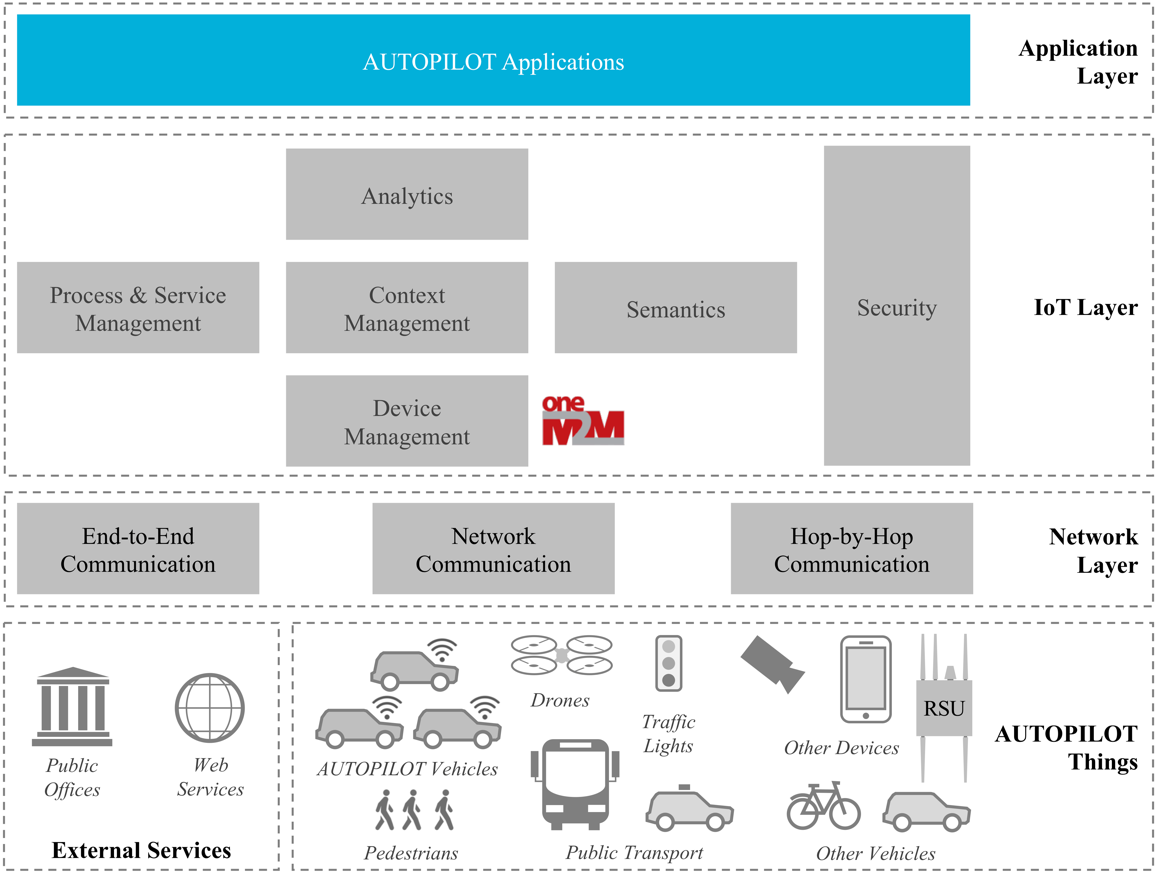
\includegraphics[width=\textwidth/5*4]{images/autopilot_layers.png}

\textsuperscript{Figure 2.6.1 Autopilot layers}\\
\textsuperscript{Retrieved from \cite{5}}
\end{figure}
%ITS 19

The second layer is the ``Network layer'', which enables communication throughout the whole IoT ecosystem. It offers three different way of communication. End-To-End Communication, which routes data packets through various parts in the network till it reaches its destination. Alternatively Hop-by-Hop Communication can be used, which specifically defines each hop (IP Address) that should be part of the path starting from the origin ending with the destination. Also communication only within a Network is possible. \textsuperscript{cmp.\cite{5}}

Third there is the ``ioT'' layer''. This layer enables the IoT functionalities. For that there are different building blocks - analytics, process and service management, context management, semantics, device management and security. They all have different functionalities and tasks to full fill with the data and the IoT Devices. \textsuperscript{cmp.\cite{5}}

Last the fourth layer is the Application layer. This layer contains the services described above itself, like car sharing or platooning. \textsuperscript{cmp.\cite{28}}

%ITS 19

The project discussed in this work dealt with the car sharing service developed in the IBM Dublin Research Lab. Car Sharing services are already a popular service in nowadays world of mobility. The services task can be either to find the closes available car for a customer and assign i or to drive the closest car directly to the customer. Then it is either possible to share a ride with other customers or with explicitly stated drivers or where the customer gets a car assigned, which he can use for himself for a given period of time.

In the future there will be one more possibility - to get the vehicle to the customer without the need of a driver but with an autonomous driving car. The car sharing service of the Autopilot app should enable this possibility combined with all the features of the IoT environment like traffic information. For that the service only needs to know the location of the customer and his origin as well as his destination and the time for which he is looking for a ride. Also the customer can enter if he wants to drive alone or if he is willing to share a ride. The car sharing service will then compute the costs and the times of the ride and match a car to a customer, which will pick him up and drop him off at his destination.

For handling all necessary informations the architecture shown in figure 2.6.2 is build for. In the central point there is the car sharing scheduler itself. This scheduler listens to an Apache Kafka client to the book topic. For this topic the customer can produce messages, for example via an app. Then the car sharing scheduler is looking for available cars through subscribing to the positions of the car in the Watson IoT Platform. To this platform vehicles publish their position and other important information like boarded customers, destinations and so on. Then it calculate the optimal route with the help of OSRM described in chapter 2.4. For that OSRM also integrates the Events published to the Watson IoT Platform. Those events can come from other IoT Vehicles, cameras, webservices or other traffic information systems like sensors or traffic lights. After the calculation of the optimal route the scheduler summon the car to the position of the customer to pick him up and take him to his destination. For that it publishes the command to the Watson IoT platform. The car subscribes to this type of information, registers the command and execute the order. Also the scheduler produces a confirmation message to the Kafka client, so that the customer can see on his app, that his ride is successfully booked. At the same time all the executed procedures are logged to a MongoDB.

\begin{figure}[h]
\centering
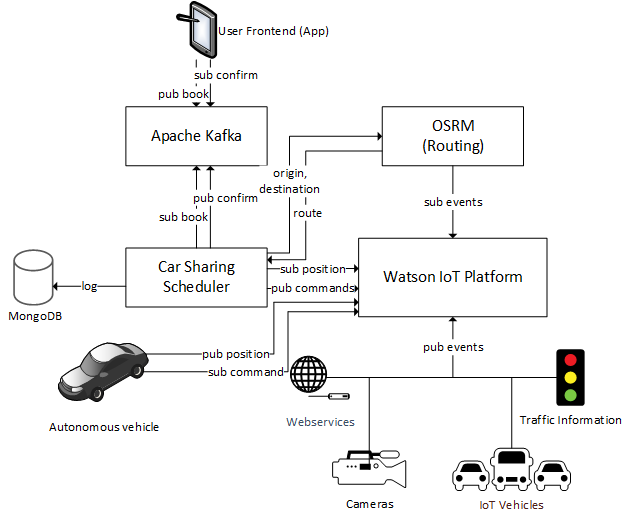
\includegraphics[width=\textwidth/5*4]{images/car_sharing_architecture.png}

\textsuperscript{Figure 2.6.2 DRL Car Sharing App Architecture}\\
\textsuperscript{Internal Source}
\end{figure}

This enables a very flexible way of a car sharing service combined with a well informed system through the IoT platform, which helps finding the best way to a specific destination. In the future this way of mobility will become more and more important, because the parking situation in cities will be even more difficult and not everybody can afford a car for his own. That's why sharing cars is a very popular way already nowadays and will become even more popular in the future.  \textsuperscript{cmp.\cite{37}}

%initial specification

%- conclusion